\documentclass[border=5pt]{standalone}
\usepackage{amsmath}
\usepackage{tikz}
\usetikzlibrary{arrows.meta,positioning,shapes.geometric,fit}
\usepackage{times}

\begin{document}
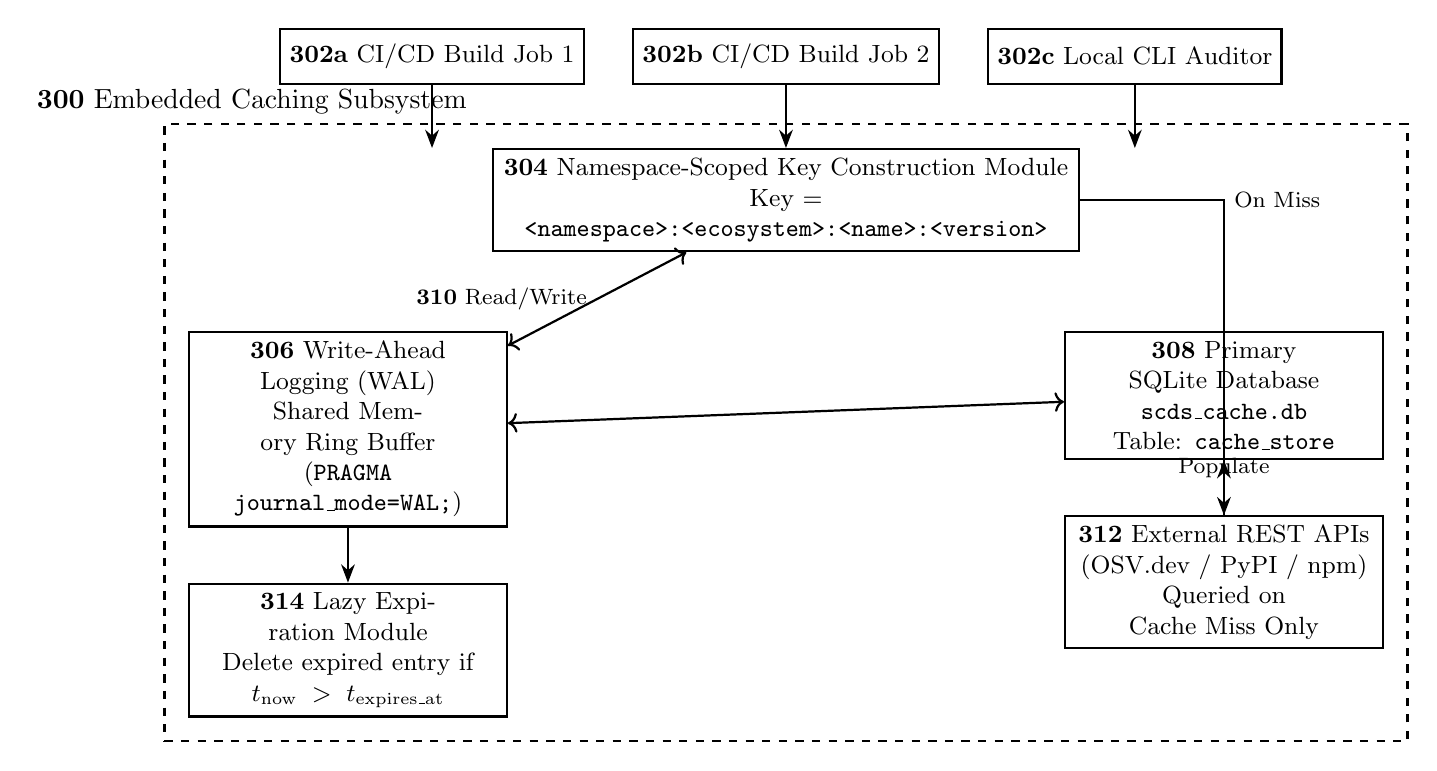
\begin{tikzpicture}[
    node distance=0.8cm and 0.8cm,
    box/.style={rectangle, draw=black, thick, fill=white, minimum height=0.7cm, align=center, font=\small},
    arrow/.style={-{Stealth[scale=1.0]}, thick, draw=black},
    group/.style={rectangle, draw=black, dashed, thick, inner sep=0.3cm, font=\small}
]

% Concurrent Processes
\node[box] (ci1) {\textbf{302a} CI/CD Build Job 1};
\node[box, right=0.6cm of ci1] (ci2) {\textbf{302b} CI/CD Build Job 2};
\node[box, right=0.6cm of ci2] (ci3) {\textbf{302c} Local CLI Auditor};

% Key Constructor
\node[box, below=0.8cm of ci2, text width=7.2cm] (keymod) {
    \textbf{304} Namespace-Scoped Key Construction Module\\
    Key = \texttt{<namespace>:<ecosystem>:<name>:<version>}
};

\draw[arrow] (ci1) -- (keymod.north -| ci1);
\draw[arrow] (ci2) -- (keymod.north);
\draw[arrow] (ci3) -- (keymod.north -| ci3);

% WAL Caching Core
\node[box, below left=1.0cm and -0.2cm of keymod, text width=3.8cm] (wal) {
    \textbf{306} Write-Ahead Logging (WAL)\\
    Shared Memory Ring Buffer\\
    (\texttt{PRAGMA journal\_mode=WAL;})
};

\node[box, below right=1.0cm and -0.2cm of keymod, text width=3.8cm] (db) {
    \textbf{308} Primary SQLite Database\\
    \texttt{scds\_cache.db}\\
    Table: \texttt{cache\_store}
};

\draw[<->, thick] (keymod) -- node[left, font=\footnotesize] {\textbf{310} Read/Write} (wal);
\draw[<->, thick] (wal) -- (db);

% Lazy Expiry Module
\node[box, below=0.7cm of wal, text width=3.8cm] (lazy) {
    \textbf{314} Lazy Expiration Module\\
    Delete expired entry if\\
    $t_{\text{now}} > t_{\text{expires\_at}}$
};
\draw[arrow] (wal) -- (lazy);

% Upstream API
\node[box, below=0.7cm of db, text width=3.8cm] (upstream) {
    \textbf{312} External REST APIs\\
    (OSV.dev / PyPI / npm)\\
    Queried on Cache Miss Only
};
\draw[arrow] (keymod) -| node[right, font=\footnotesize] {On Miss} (upstream);
\draw[arrow] (upstream) -- node[above, font=\footnotesize] {Populate} (db);

% Overall Cache Subsystem
\node[group, fit=(keymod) (wal) (db) (lazy), label=above left:{\textbf{300} Embedded Caching Subsystem}] (cachesys) {};

\end{tikzpicture}
\end{document}
